\documentclass[a4paper]{article}
\usepackage[utf8]{inputenc}
\usepackage[russian]{babel}
\usepackage[T2]{fontenc}
\usepackage[warn]{mathtext}
\usepackage{graphicx}
\usepackage{amsmath}
\usepackage{floatflt}
\usepackage[left=20mm, top=20mm, right=20mm, bottom=20mm, footskip=10mm]{geometry}


\graphicspath{ {images/} }
\usepackage{multicol}
\setlength{\columnsep}{2cm}


\begin{document}

\begin{titlepage}
	\centering
	\vspace{5cm}
	{\scshape\LARGE Московский физико-технический институт \par}
	\vspace{4cm}
	{\scshape\Large Лабораторная работа \par}
	\vspace{1cm}
	{\huge\bfseries Исследование разрешающей способности микроскопа методом Аббе \par}
	\vspace{1cm}
	\vfill
\begin{flushright}
	{\large выполнили студенты 653 группы ФФКЭ}\par
	\vspace{0.3cm}
	{\LARGE Карпова Татьяна} \par
		\vspace{0.3cm}
	{\LARGE Давыдов Валентин}
\end{flushright}
	

	\vfill

% Bottom of the page
	Долгопрудный, 2018 г.
\end{titlepage}

\section{Цель работы:}
Определение дифракционного предела разрешения
объектива микроскопа методом Аббе.

\section{В работе используются:}
\begin{itemize}
    \item лазер
    \item кассета с набором сеток разного
периода
    \item линзы
    \item щель с микрометрическим винтом
    \item оптический стол
c набором рейтеров и крепёжных винтов
    \item экран
    \item линейка
\end{itemize}

\section{Теоретические положения}

Разрешающей способностью оптического прибора называют минимальное расстояние $l_{min}$ между двумя точками в пространстве предметов, которое прибор может разрешить. При визуальном наблюдении изображения в качестве критерия разрешения применяют так называемый критерий Рэлея. \par
Для иммерсионного микроскопа (объект находится в иммерсионной среде — жидкости с показателем преломления n) разрешающая способность объектива при некогерентном освещении
\begin{equation}
    l_{min} = \frac{0.61 \lambda}{n \sin A},
\end{equation}

где A — апертурный угол объектива микроскопа. \par
Рассмотрим теперь когерентно освещённый объект, наблюдаемый в микроскоп. Схема образования изображения в объективе микроскопа
представлена на рис. 1.
    \begin{figure}[h]
    \centering
    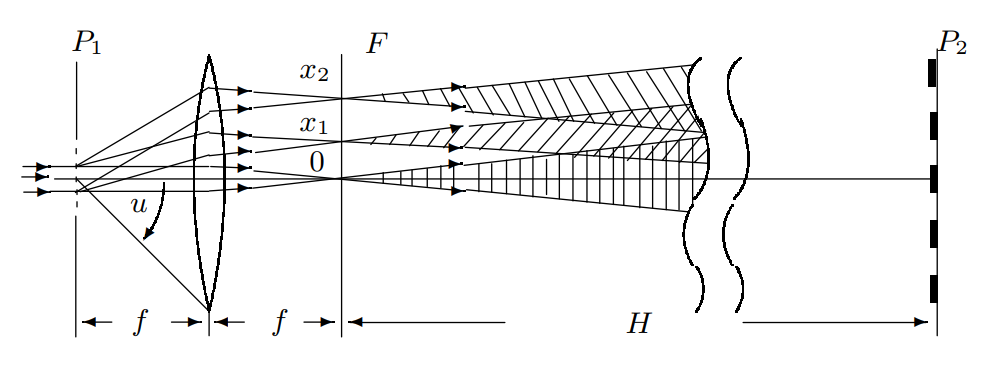
\includegraphics[width=15cm]{fig2.PNG}
    \caption{Образование изображения в объективе микроскопа. $P_1$ — плоскость предмета, $F$ — задняя фокальная плоскость объектива, $P_2$ — плоскость,
сопряжённая с предметной плоскостью. В плоскости $P_2$ световые пучки
сильно перекрываются}
    \label{fig:vac}
\end{figure}

минимальное разрешаемое объективом расстояние
определяется условием

\begin{equation}
    l_{min} = \frac{\lambda}{\sin A} \approx \frac{\lambda}{D/2f},
\end{equation}

где D — диаметр диафрагмы. При этом диафрагма, расположенная
симметрично, пропускает нулевой и ±1 дифракционные максимумы.


\section{Экспериментальная установка}

Схема модели проекционного микроскопа приведена на рис. 2. Предметом служат сетки, расположенные
в кассете. Смена сеток осуществляется поворотом внешнего кольца кассеты.

    \begin{figure}[h]
    \centering
    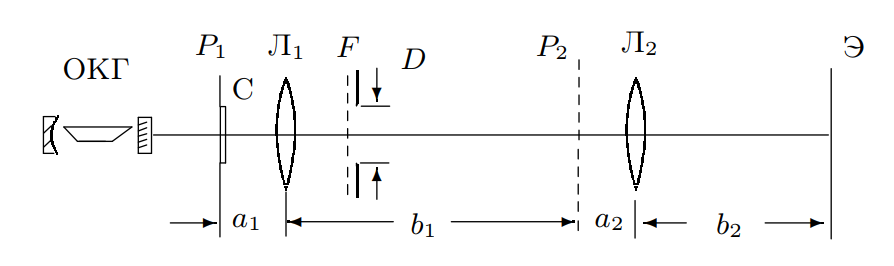
\includegraphics[width=15cm]{fig1.PNG}
    \caption{Схема экспериментальной установки — модель проекционного
микроскопа}
    \label{fig:vac}
\end{figure}

\section{Ход работы}
\subsection{Определение периода решёток по их пространственному спектру}
\begin{enumerate}
    \item Для определения периода решёток измерим расстояния между максимумами разных порядков на экране. Расстояние от сетки до экрана $D = 141.5$ см. Период решётки рассчитывается по формуле 
    \begin{equation}
        d = \frac{\lambda D}{d_{mes}}
    \end{equation}
    Результаты измерений занесём в таблицу 1.
    
        \begin{table}[h]
    \centering
    \begin{center}
    \caption{Периоды решёток, метод пространственного спектра}
    \end{center}
    \vspace{0.1cm}
    \label{tab:my_label}
    \begin{tabular}{ |p{2.5cm}||p{1cm}|p{1cm}|p{1cm}|p{1cm}|p{1cm}|}
 \hline
Номер решётки & 1 & 2 & 3 & 4 & 5\\
 \hline
 $d_{mes}$, см & 3.625 & 2.5 & 1.257 & 0.625 & 0.455 \\
 \hline
 $d$, мкм & 20.676 & 30.111 & 59.887 & 120.445 & 165.446\\

 \hline
 
\end{tabular}
\end{table}
\end{enumerate}

\subsection{Определение периода решёток по изображению, увеличенному
с помощью модели микроскопа}
\begin{enumerate}
    \item Соберём модель проекционного микроскопа (рис. 2), центрируем систему. Увеличение полученной системы вычисляется по формуле
    \begin{equation}
        \gamma = \frac{a_1}{b_1+b_2+a_2},
    \end{equation}
    (расстояния $a_1$, $a_2$, $b_1$, $b_2$ см на рис. 2)
    \item На экране измерим расстояния между максимумами разных порядков. Результаты измерений занесём в таблицу 2.
    
        \begin{table}[h]
    \centering
    \begin{center}
    \caption{Периоды решёток, по изображению с микроскопа}
    \end{center}
    \vspace{0.1cm}
    \label{tab:my_label}
    \begin{tabular}{ |p{2.5cm}||p{1cm}|p{1cm}|p{1cm}|p{1cm}|}
 \hline
Номер решётки & 2 & 3 & 4 & 5\\
 \hline
 $d_{mes}$, мм & 0.293 & 0.609 & 1.156 & 1.64 \\
 \hline
 $d$, мкм & 34.07 & 70.814 & 135.465 & 191.698 \\

 \hline
 
\end{tabular}
\end{table}

\end{enumerate}

\subsection{Определение периодов решёток по оценке разрешающей способности микроскопа}
\begin{enumerate}
    \item Поместим щелевую диафрагму с микрометрическим винтом в фокальную плоскость $F$ линзы Л1. Определите для каждой решётки минимальный размер диафрагмы $D$, при котором на экране ещё видно изображение сетки (при меньших размерах щели изображение выглядит
как одномерная решётка). Результаты измерений занесём в таблицу 3.

        \begin{table}[h]
    \centering
    \begin{center}
    \caption{Периоды решёток, по измерению диафрагмы}
    \end{center}
    \vspace{0.1cm}
    \label{tab:my_label}
    \begin{tabular}{ |p{2.5cm}||p{1cm}|p{1cm}|p{1cm}|}
 \hline
Номер решётки &  3 & 4 & 5\\
 \hline
 $D$, мм  & 2.78 & 1.12 & 0.87 \\
 \hline
 $d$, мкм  & 55.496 & 137.75 & 177.333 \\

 \hline
 
\end{tabular}
\end{table}

    \begin{figure}[h]
    \centering
    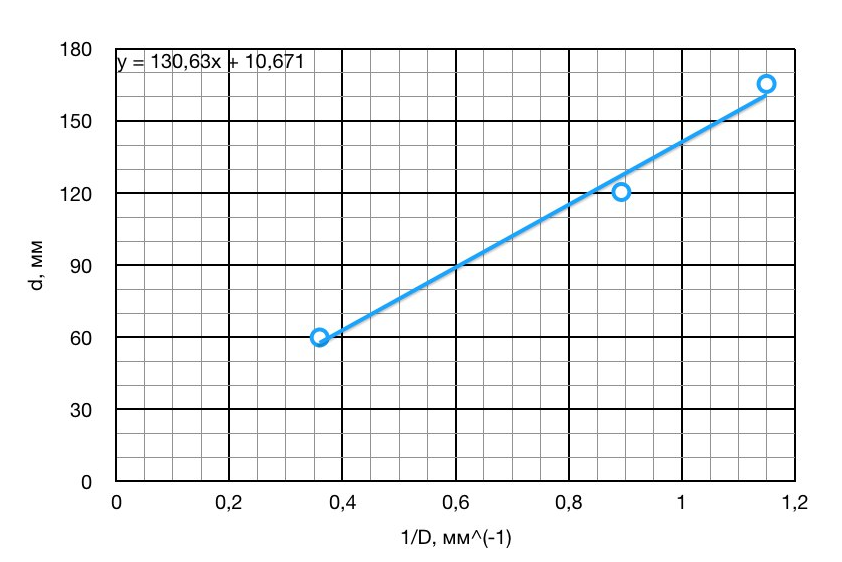
\includegraphics[width=13cm]{fig3.PNG}
    \caption{Зависимость d = f(1/D)}
    \label{fig:vac}
\end{figure}

\item Для проверки теории Аббе построим график зависимости d = f(1/D), взяв периоды сеток, определённые по спектру. Определим угловой коэффициент, он равен 130. По формуле $d \ge \frac{\lambda}{D/2f}$, тогда при наших условиях теоретический угловой коэффициент равен 154. Теория Аббе верна в пределах используемой точности.

\end{enumerate}

\subsection{Пространственная фильтрация и мультиплицирование}

Поворачивая щель относительно оси, добьёмся того, чтобы щель занимала наклонное положение под $45^\circ$. Тогда будет осуществляться пространственная фильтрация, то есть выделение из спектра максимумов $m_x = m_y$ (диагональных максимумов). Тогда на экране возникнет изображение решётки, которой нет на самом деле. Полосы располагаются под углом $45^\circ$, что видно на рисунке \ref{filtr}. Период новой решетки равен 0,852 мм, что в $\sqrt{2}$ раз больше периода изображения решётки, определённого стандартным методом (по увеличенному изображению решётки). Это объясняется тем фактом, что расстояние между выделенными максимумами, то есть между вторичными источниками волн, составляет $d\sqrt{2}$. Также наблюдали мультиплицирование, то есть рассечение фурье-образа щели сеткой. Такой эффект создаётся, если в нашей установке поменять местами сетку и щель.

\begin{figure}[h]
    \centering
    \includegraphics[width=8cm]{LabPhotoBestProject.jpg}
    \caption{Пространственная фильтрация}
    \label{filtr}
\end{figure}

\section{Вывод}

В ходе работы были измерены периоды различных дифракционных решёток тремя различными способами: по пространственному спектру, изображению с микроскопа и по оценке разрешающей способности микроскопа. Результаты измерений практически совпадают. Сравнение результатов, полученных разными методами, приведено в таблице 4. 

Также в работе наблюдалось и объяснялось явление пространственной фильтрации и мультиплицирования. Фактически проводилась работа с фурье-образами щели и сетки, то есть выделение и рассечение образа.

     \begin{table}[h]
    \centering
    \begin{center}
    \caption{Периоды решёток, различные методы}
    \end{center}
    \vspace{0.1cm}
    \label{tab:my_label}
    \begin{tabular}{ |p{4cm}||p{1.2cm}|p{1.2cm}|p{1.2cm}|p{1.2cm}|p{1.2cm}|}
 \hline
Номер решётки & 1 & 2 & 3 & 4 & 5\\
 \hline
 $d$, мкм - простр. спектр  & 20.676 & 30.111 & 59.887 & 120.445 & 165.446 \\
 \hline
 $d$, мкм - микроскоп & - & 34.07 & 70.814 & 135.465 & 191.698 \\
 \hline
 $d$, мкм - диафрагма  & - & - & 55.496 & 137.75 & 177.333 \\

 \hline
 
\end{tabular}
\end{table}   


\end{document}
